% Options for packages loaded elsewhere
\PassOptionsToPackage{unicode}{hyperref}
\PassOptionsToPackage{hyphens}{url}
\PassOptionsToPackage{dvipsnames,svgnames,x11names}{xcolor}
%
\documentclass[
  letterpaper,
  DIV=11,
  numbers=noendperiod]{scrartcl}

\usepackage{amsmath,amssymb}
\usepackage{iftex}
\ifPDFTeX
  \usepackage[T1]{fontenc}
  \usepackage[utf8]{inputenc}
  \usepackage{textcomp} % provide euro and other symbols
\else % if luatex or xetex
  \usepackage{unicode-math}
  \defaultfontfeatures{Scale=MatchLowercase}
  \defaultfontfeatures[\rmfamily]{Ligatures=TeX,Scale=1}
\fi
\usepackage{lmodern}
\ifPDFTeX\else  
    % xetex/luatex font selection
\fi
% Use upquote if available, for straight quotes in verbatim environments
\IfFileExists{upquote.sty}{\usepackage{upquote}}{}
\IfFileExists{microtype.sty}{% use microtype if available
  \usepackage[]{microtype}
  \UseMicrotypeSet[protrusion]{basicmath} % disable protrusion for tt fonts
}{}
\makeatletter
\@ifundefined{KOMAClassName}{% if non-KOMA class
  \IfFileExists{parskip.sty}{%
    \usepackage{parskip}
  }{% else
    \setlength{\parindent}{0pt}
    \setlength{\parskip}{6pt plus 2pt minus 1pt}}
}{% if KOMA class
  \KOMAoptions{parskip=half}}
\makeatother
\usepackage{xcolor}
\setlength{\emergencystretch}{3em} % prevent overfull lines
\setcounter{secnumdepth}{4}
% Make \paragraph and \subparagraph free-standing
\makeatletter
\ifx\paragraph\undefined\else
  \let\oldparagraph\paragraph
  \renewcommand{\paragraph}{
    \@ifstar
      \xxxParagraphStar
      \xxxParagraphNoStar
  }
  \newcommand{\xxxParagraphStar}[1]{\oldparagraph*{#1}\mbox{}}
  \newcommand{\xxxParagraphNoStar}[1]{\oldparagraph{#1}\mbox{}}
\fi
\ifx\subparagraph\undefined\else
  \let\oldsubparagraph\subparagraph
  \renewcommand{\subparagraph}{
    \@ifstar
      \xxxSubParagraphStar
      \xxxSubParagraphNoStar
  }
  \newcommand{\xxxSubParagraphStar}[1]{\oldsubparagraph*{#1}\mbox{}}
  \newcommand{\xxxSubParagraphNoStar}[1]{\oldsubparagraph{#1}\mbox{}}
\fi
\makeatother


\providecommand{\tightlist}{%
  \setlength{\itemsep}{0pt}\setlength{\parskip}{0pt}}\usepackage{longtable,booktabs,array}
\usepackage{calc} % for calculating minipage widths
% Correct order of tables after \paragraph or \subparagraph
\usepackage{etoolbox}
\makeatletter
\patchcmd\longtable{\par}{\if@noskipsec\mbox{}\fi\par}{}{}
\makeatother
% Allow footnotes in longtable head/foot
\IfFileExists{footnotehyper.sty}{\usepackage{footnotehyper}}{\usepackage{footnote}}
\makesavenoteenv{longtable}
\usepackage{graphicx}
\makeatletter
\def\maxwidth{\ifdim\Gin@nat@width>\linewidth\linewidth\else\Gin@nat@width\fi}
\def\maxheight{\ifdim\Gin@nat@height>\textheight\textheight\else\Gin@nat@height\fi}
\makeatother
% Scale images if necessary, so that they will not overflow the page
% margins by default, and it is still possible to overwrite the defaults
% using explicit options in \includegraphics[width, height, ...]{}
\setkeys{Gin}{width=\maxwidth,height=\maxheight,keepaspectratio}
% Set default figure placement to htbp
\makeatletter
\def\fps@figure{htbp}
\makeatother
% definitions for citeproc citations
\NewDocumentCommand\citeproctext{}{}
\NewDocumentCommand\citeproc{mm}{%
  \begingroup\def\citeproctext{#2}\cite{#1}\endgroup}
\makeatletter
 % allow citations to break across lines
 \let\@cite@ofmt\@firstofone
 % avoid brackets around text for \cite:
 \def\@biblabel#1{}
 \def\@cite#1#2{{#1\if@tempswa , #2\fi}}
\makeatother
\newlength{\cslhangindent}
\setlength{\cslhangindent}{1.5em}
\newlength{\csllabelwidth}
\setlength{\csllabelwidth}{3em}
\newenvironment{CSLReferences}[2] % #1 hanging-indent, #2 entry-spacing
 {\begin{list}{}{%
  \setlength{\itemindent}{0pt}
  \setlength{\leftmargin}{0pt}
  \setlength{\parsep}{0pt}
  % turn on hanging indent if param 1 is 1
  \ifodd #1
   \setlength{\leftmargin}{\cslhangindent}
   \setlength{\itemindent}{-1\cslhangindent}
  \fi
  % set entry spacing
  \setlength{\itemsep}{#2\baselineskip}}}
 {\end{list}}
\usepackage{calc}
\newcommand{\CSLBlock}[1]{\hfill\break\parbox[t]{\linewidth}{\strut\ignorespaces#1\strut}}
\newcommand{\CSLLeftMargin}[1]{\parbox[t]{\csllabelwidth}{\strut#1\strut}}
\newcommand{\CSLRightInline}[1]{\parbox[t]{\linewidth - \csllabelwidth}{\strut#1\strut}}
\newcommand{\CSLIndent}[1]{\hspace{\cslhangindent}#1}

\usepackage{booktabs}
\usepackage{longtable}
\usepackage{array}
\usepackage{multirow}
\usepackage{wrapfig}
\usepackage{float}
\usepackage{colortbl}
\usepackage{pdflscape}
\usepackage{tabu}
\usepackage{threeparttable}
\usepackage{threeparttablex}
\usepackage[normalem]{ulem}
\usepackage{makecell}
\usepackage{xcolor}
\usepackage{caption}
\usepackage{anyfontsize}
\KOMAoption{captions}{tableheading}
\makeatletter
\@ifpackageloaded{caption}{}{\usepackage{caption}}
\AtBeginDocument{%
\ifdefined\contentsname
  \renewcommand*\contentsname{Table of contents}
\else
  \newcommand\contentsname{Table of contents}
\fi
\ifdefined\listfigurename
  \renewcommand*\listfigurename{List of Figures}
\else
  \newcommand\listfigurename{List of Figures}
\fi
\ifdefined\listtablename
  \renewcommand*\listtablename{List of Tables}
\else
  \newcommand\listtablename{List of Tables}
\fi
\ifdefined\figurename
  \renewcommand*\figurename{Figure}
\else
  \newcommand\figurename{Figure}
\fi
\ifdefined\tablename
  \renewcommand*\tablename{Table}
\else
  \newcommand\tablename{Table}
\fi
}
\@ifpackageloaded{float}{}{\usepackage{float}}
\floatstyle{ruled}
\@ifundefined{c@chapter}{\newfloat{codelisting}{h}{lop}}{\newfloat{codelisting}{h}{lop}[chapter]}
\floatname{codelisting}{Listing}
\newcommand*\listoflistings{\listof{codelisting}{List of Listings}}
\makeatother
\makeatletter
\makeatother
\makeatletter
\@ifpackageloaded{caption}{}{\usepackage{caption}}
\@ifpackageloaded{subcaption}{}{\usepackage{subcaption}}
\makeatother

\ifLuaTeX
  \usepackage{selnolig}  % disable illegal ligatures
\fi
\usepackage{bookmark}

\IfFileExists{xurl.sty}{\usepackage{xurl}}{} % add URL line breaks if available
\urlstyle{same} % disable monospaced font for URLs
\hypersetup{
  pdftitle={Joint Coho Technical Committee Periodic Report},
  pdfauthor={PSC Joint Coho Technical Committee},
  colorlinks=true,
  linkcolor={blue},
  filecolor={Maroon},
  citecolor={Blue},
  urlcolor={Blue},
  pdfcreator={LaTeX via pandoc}}


\title{Joint Coho Technical Committee Periodic Report}
\author{PSC Joint Coho Technical Committee}
\date{2024-12-03}

\begin{document}
\maketitle

\renewcommand*\contentsname{Table of contents}
{
\hypersetup{linkcolor=}
\setcounter{tocdepth}{4}
\tableofcontents
}

!! SPLIT FROM DRAFT DOCUMENT UNDER DEVELOPMENT !!

This is split off of the periodic report (on 12/3/2024), and presents
key summaries for a specific year range. Any caveats associated with
taht version of the periodic report also apply here.

\textbf{Using data ONLY from 2019 to 2022}

\emph{Note that Quillayute and Queets values are those from the FRAM
database and have not yet been extracted from the relevant TAMM cells
for each year}

This report is based on postseason data in
PSC\_CoTC\_PostSeason\_CohoFRAMDB\_thru2022\_03042024.mdb and preseason
data in PSC\_CoTC\_Preseason\_CohoFRAMDB\_thru2024\_06182024.mdb, as
well as supporting
\href{https://github.com/PSC-CoTC/PeriodicReport/blob/master/StaticTables.xlsx}{StaticTables.xlsx}.

\includegraphics[width=1\textwidth,height=\textheight]{images/coho_pic2.png}

\section{Introduction}\label{introduction}

In response to a decline in natural Coho Salmon (\emph{Onchorynchus
kisutch}) abundance, the Pacific Salmon Commission established a
Southern Coho abundance-based management regime (CoABM) in 1999 (Pacific
Salmon Commission 1999). This Southern Coho Management Plan (SCMP, also
referred to as ABM, or `abundance based management') aimed to conserve
Coho Salmon Management Units (MUs of naturally-spawning Coho Salmon in
southern British Columbia and Washington/Oregon) based on abundance
status and escapement goals. The SCMP set out to constrain exploitation
rates (ERs; defined as total fishing mortality divided by total fishing
mortality plus escapement) below maximum levels (caps) on selected
management units in order to achieve long-term Maximum Sustainable
Harvests (MSH). These constraints are implemented by specifying ER caps
for the individual MUs dependent on annual abundance status. During
their respective preseason planning processes, the Parties use
management reference points to classify the status of each MU as low,
moderate, or abundant. The parties then exchange these status
determinations as a key input in the development of pre-season plans.

When a new Coho Management Plan was reached in 2008 (implemented 2009
through 2018; (Pacific Salmon Commission 2009)) and the latest agreement
finalized (applies to the period from catch years 2019 through 2028;
(Pacific Salmon Commission 2022)), modifications were made to the list
of specified MUs and to the manner in which exploitation rate caps are
established. This periodic report presents information for the MUs
identified in the most current Pacific Salmon Treaty's (PST) Southern
Coho Management Plan (Chapter 5 of Annex IV in the current PST). In the
2008 SCMP abundance-based management regimes were established to
constrain exploitation rates (ERs) on the 13 Management Units (MUs) of
naturally-spawning Coho Salmon originating in rivers along the
Washington/British Columbia (BC) border. Within the most recent
Management Plan (Pacific Salmon Commission 2022), two of the Canadian
MUs, the Georgia Strait Vancouver Island and the Georgia Strait Mainland
Management Units, are now combined into the Strait of Georgia Management
Unit. The 12 MUs in the current PST are listed below.

\begin{table}
\caption*{
{\large Management Units within the current Pacific Salmon Treaty Southern Coho Management Plan.}
} 
\fontsize{12.0pt}{14.4pt}\selectfont
\begin{tabular*}{300pt}{@{\extracolsep{\fill}}lll}
\toprule
{\bfseries Southern BC} & {\bfseries US Inside} & {\bfseries US Outside} \\ 
\midrule\addlinespace[2.5pt]
{Interior Fraser} & {Skagit} & {Quillayute} \\ 
{Lower Fraser} & {Stillaguamish} & {Hoh} \\ 
{Georgia Strait Vancouver Island} & {Snohomish} & {Queets} \\ 
{Georgia Strait Mainland} & {Hood Canal} & {Grays Harbor} \\ 
{} & {US Strait JDF} & {} \\ 
\bottomrule
\end{tabular*}
\end{table}

The objective of the SCMP, as described in the Treaty, is to manage the
fisheries impact on Southern Coho stocks by limiting the total fishery
exploitation and allow the different MUs to produce long-term Maximum
Sustainable Harvest (MSH), while maintaining the genetic and ecological
diversity of the individual populations. In addition, the plan is
designed to improve the prospect of sustaining healthy fisheries for
both parties over the long-term. The plan is intended to be
cost-effective and flexible to available technical capacity and
information, while providing a predictable framework for planning
fisheries impacts and allowing for objective monitoring, evaluation and
modification.

Under the Agreement, the Parties are required to establish escapement
goals or ERs that achieve MSH, determine MSH ERs for each MU, and
establish ERs for each MU and status category (low, moderate, and
abundant). Until such time as the Parties provide MU-specific ER
targets, the SCMP identified default ER ceilings for the following MU
status categories:

\begin{longtable}[]{@{}cc@{}}
\toprule\noalign{}
\textbf{Status} & \textbf{Total Exploitation Rate} \\
\midrule\noalign{}
\endhead
\bottomrule\noalign{}
\endlastfoot
Low & Up to 20\% \\
Moderate & 21\% - 40\% \\
Abundant & 41\% - 65\% \\
\end{longtable}

Annual ER caps are established for each of the MUs based on the level of
abundance and health of the natural stocks. These caps are then
apportioned between the Parties. Constraints for Canadian fisheries on
US MUs are determined by formulas that specify sharing of allowable ERs
as well as a composite rule, which together adjust caps according to the
number of US MUs that fall within a given category. The composite rule
adjusts constraints for Canadian fishery exploitation rates based on the
number of US management units which fall in a given category. For
example, if only one Washington coastal or Puget Sound Coho management
unit is in low status, Canadian fisheries are constrained to a total
exploitation rate on that unit of 12\%; if two or more Washington
coastal management units are in low status, the constraint becomes 10\%.
The most restrictive exploitation rate limit for Canadian fishery
impacts on US Coho management units is 10\%.

Constraints for US fisheries on Canadian MUs depend on the status of the
Interior Fraser MU until the biological statuses of the other Canadian
MUs have been determined. The status determination methodology developed
and applied by Canada to the Interior Fraser Coho MU (REFERENCE Korman
and Sawada) consists of two criteria: smolt-to-adult survival, and
escapement, which must be met for three consecutive years in order
increase the status from low to moderate or moderate to high. Canada is
currently working to develop the information (smolt to adult survival
rates, escapements) needed to apply this status determination
methodology to the Lower Fraser and Strait of Georgia MUs. Details as to
how exploitation rate constraints are established based on the status of
MUs under the SCMP are contained in Annex IV Chapter 5 Section 9.b-c
(Canadian exploitation rate caps on inside and outside US MUs) and
Section 9.d (US exploitation rate caps on Canadian MUs).

\subsection{Management Unit Overview}\label{management-unit-overview}

The Canadian MUs are comprised of geographical aggregates of naturally
spawning Coho conservation units (CUs) within the Interior Fraser River,
Lower Fraser River, and Strait of Georgia. A CU consists of one or more
spawning populations which are genetically distinct from other
conspecific spawning populations. The 2019 renewal of the PST combined
the Georgia Basin -- East and Georgia Basin -- West MUs into a single
Strait of Georgia MU, reducing the number of Canadian MUs in the
bilateral management regime to three. The CoTC chose to combine model
outputs for these MUs in carrying out its pre-season and post-season
responsibilities beginning in 2019 and forward rather than reconfigure
the FRAM framework.

The US Inside MUs consist of naturally spawning populations originating
in the Skagit, Stillaguamish, Snohomish, Hood Canal, and the Strait of
Juan de Fuca. Coho populations in the US Inside MUs belong to the larger
Puget Sound/Strait of Georgia Coho Salmon evolutionarily significant
unit (ESU; (Weitkamp et al. 1995)). Only the eastern portion of the
Strait of Juan de Fuca MU is in this ESU. An ESU is a Pacific salmon
population or group of populations that is substantially reproductively
isolated from other conspecific populations and represents an important
component of the evolutionary legacy of the species. The ESU policy (56
FR 58612) for Pacific salmon defines the criteria for identifying a
Pacific salmon population as a distinct population segment, which can be
listed under the US Endangered Species Act of 1973.

The US Outside MUs consist of naturally-spawning populations from the
Quillayute, Hoh, Queets, and Grays Harbor basins. All US Outside MUs,
except the Grays Harbor MU, are part of the Olympic Peninsula ESU.
Populations from the western portion of the Strait of Juan de Fuca MU
are also in this ESU. The Grays Harbor MU is part of the Southwest
Washington ESU.

\begin{table}
\caption*{
{\large Management Units within the current Pacific Salmon Treaty Southern Coho Management Plan}
} 
\fontsize{12.0pt}{14.4pt}\selectfont
\begin{tabular*}{300pt}{@{\extracolsep{\fill}}lll}
\toprule
{\bfseries Southern BC} & {\bfseries US Inside} & {\bfseries US Outside} \\ 
\midrule\addlinespace[2.5pt]
{Interior Fraser} & {Skagit} & {Quillayute} \\ 
{Lower Fraser} & {Stillaguamish} & {Hoh} \\ 
{Strait of Georgia} & {Snohomish} & {Queets} \\ 
{} & {Hood Canal} & {Grays Harbor} \\ 
{} & {US Strait JDF} & {} \\ 
\bottomrule
\end{tabular*}
\end{table}

\section{Performance of Abundance Based Management
Regime}\label{performance-of-abundance-based-management-regime}

In an attempt to evaluate the implementation of Abundance Based
Management of Coho Salmon stocks of concern under the PST, summaries on
abundance categories, exploitation, and forecast performance are
provided below. Catch years summarized include 2004 through 2021 and
abundance category and forecast performance summaries are limited to US
and Interior Fraser River MUs. A single year of post-season estimates of
MU abundances, fishery exploitation, and escapement is first completed
two years following each catch year. For example, an assessment of catch
year 2022 will be completed in February of 2024. This report has been
referred to as the Annual ER Report. This assessment is presented to the
Southern Panel at the PSC's Annual Meeting and the reports are posted on
the CoTC's and Southern Panel's Sharepoint sites. These annual reports
can also be found \emph{here}. The best available data and the most
current FRAM base period and Terminal Area Management Modules (TAMMs)
are used to evaluate the catch year; however, data and the FRAM base
period is updated or corrected on occasion. These corrections and
additions are carried forward and are included in the post-season
evaluations of MUs below, sometimes resulting in changes from the annual
reports in estimates of exploitation rates, escapement numbers, and
Ocean Age-3 abundances.

\subsection{Management Unit Post-season Abundances and
Categories}\label{management-unit-post-season-abundances-and-categories}

Currently all of the MUs except the Lower Fraser River and Georgia
Strait MUs have abundance break point criteria and associated
exploitation rates for each abundance category. A summary of MU
abundances and associated categories are provided in the following table
and figure.

** Post-season estimates of Ocean Age-3 total abundances and their
associated status categories {[}A = abundant, M = moderate, L= low{]} by
MU for catch years 2004 through 2021. Management Units in the Abundant
category have green highlighted cells, Moderate ones are not
highlighted, and those in Low status are highlighted orange.** (note -
need to make table fit unto a single page in Word)

\begin{table}
\fontsize{12.0pt}{14.4pt}\selectfont
\begin{tabular*}{1125pt}{@{\extracolsep{\fill}}>{\raggedright\arraybackslash}p{\dimexpr 112.50pt -2\tabcolsep-1.5\arrayrulewidth}rr>{\raggedleft\arraybackslash}p{\dimexpr 90.00pt -2\tabcolsep-1.5\arrayrulewidth}>{\raggedleft\arraybackslash}p{\dimexpr 90.00pt -2\tabcolsep-1.5\arrayrulewidth}>{\raggedleft\arraybackslash}p{\dimexpr 90.00pt -2\tabcolsep-1.5\arrayrulewidth}>{\raggedleft\arraybackslash}p{\dimexpr 90.00pt -2\tabcolsep-1.5\arrayrulewidth}}
\toprule
PSC\_StockName & low\_mod\_abund & mod\_abd\_abund & {\bfseries \cellcolor[HTML]{B3B3B3}{2019}} & {\bfseries \cellcolor[HTML]{B3B3B3}{2020}} & {\bfseries \cellcolor[HTML]{B3B3B3}{2021}} & {\bfseries \cellcolor[HTML]{B3B3B3}{2022}} \\ 
\midrule\addlinespace[2.5pt]
\multicolumn{7}{>{\raggedright\arraybackslash}m{1125pt}}{Canada} \\[2.5pt] 
\midrule\addlinespace[2.5pt]
Lower Fraser & NA & NA & 42,572 & 85,395 & 47,539 & 78,093 \\ 
Interior Fraser & NA & NA & 54,777 & 82,191 & 87,210 & 80,129 \\ 
Strait of Georgia & NA & NA & 32,727 & 109,574 & 140,232 & 128,444 \\ 
\midrule\addlinespace[2.5pt]
\multicolumn{7}{>{\raggedright\arraybackslash}m{1125pt}}{US Inside} \\[2.5pt] 
\midrule\addlinespace[2.5pt]
Skagit & 22857 & 62500 & 27,499 [M] & 41,468 [M] & {\cellcolor[HTML]{C6F5BA}{111,989 [A]}} & {\cellcolor[HTML]{C6F5BA}{124,042 [A]}} \\ 
Stillaguamish & 9385 & 20000 & 16,165 [M] & {\cellcolor[HTML]{C6F5BA}{24,654 [A]}} & {\cellcolor[HTML]{C6F5BA}{42,702 [A]}} & {\cellcolor[HTML]{C6F5BA}{59,711 [A]}} \\ 
Snohomish & 51667 & 125000 & {\cellcolor[HTML]{F5E298}{48,671 [L]}} & {\cellcolor[HTML]{F5E298}{47,717 [L]}} & 109,873 [M] & 93,201 [M] \\ 
Hood Canal & 19545 & 41000 & {\cellcolor[HTML]{F5E298}{14,666 [L]}} & 23,616 [M] & {\cellcolor[HTML]{C6F5BA}{45,719 [A]}} & 20,007 [M] \\ 
US Strait JDF & 11679 & 27445 & {\cellcolor[HTML]{F5E298}{5,258 [L]}} & {\cellcolor[HTML]{F5E298}{9,200 [L]}} & 22,440 [M] & 18,396 [M] \\ 
\midrule\addlinespace[2.5pt]
\multicolumn{7}{>{\raggedright\arraybackslash}m{1125pt}}{US Outside} \\[2.5pt] 
\midrule\addlinespace[2.5pt]
Quillayute & 7875 & 10500 & {\cellcolor[HTML]{C6F5BA}{10,905 [A]}} & 9,107 [M] & {\cellcolor[HTML]{C6F5BA}{11,578 [A]}} & {\cellcolor[HTML]{C6F5BA}{16,266 [A]}} \\ 
Hoh & 2500 & 3333 & {\cellcolor[HTML]{C6F5BA}{5,157 [A]}} & {\cellcolor[HTML]{C6F5BA}{5,386 [A]}} & {\cellcolor[HTML]{C6F5BA}{7,790 [A]}} & {\cellcolor[HTML]{C6F5BA}{11,686 [A]}} \\ 
Queets & 7250 & 9667 & {\cellcolor[HTML]{F5E298}{3,944 [L]}} & {\cellcolor[HTML]{F5E298}{5,126 [L]}} & {\cellcolor[HTML]{F5E298}{5,261 [L]}} & {\cellcolor[HTML]{C6F5BA}{17,811 [A]}} \\ 
Grays Harbor & 44250 & 59000 & 50,994 [M] & {\cellcolor[HTML]{F5E298}{31,581 [L]}} & {\cellcolor[HTML]{C6F5BA}{77,315 [A]}} & {\cellcolor[HTML]{C6F5BA}{79,356 [A]}} \\ 
\bottomrule
\end{tabular*}
\end{table}

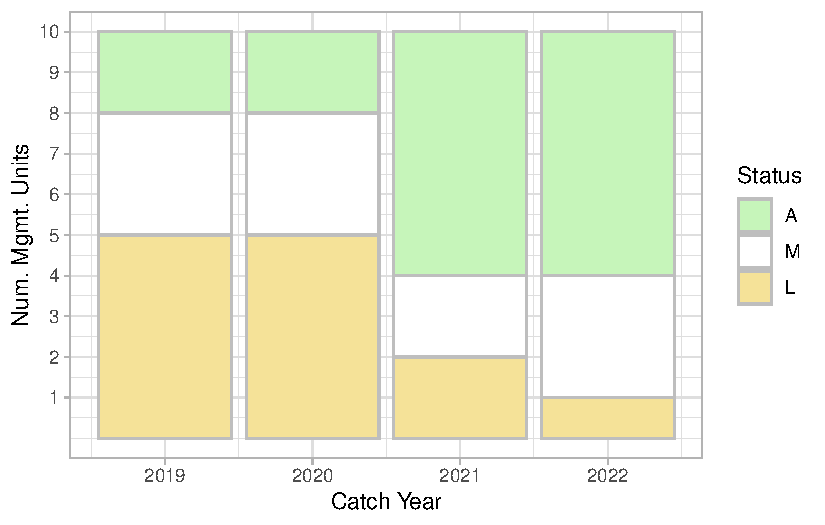
\includegraphics{index-5yr_files/figure-pdf/fig_unit_status_stackedcol-1.pdf}

Estimated post-season ocean age-3 cohort abundances for the MUs are
depicted below. Abundances for BC and US Inside MUs tend to be
synchronous, with above- or below-average abundances occurring in the
same years (e.g., high in 2001, low in 2006). Outside MUs are less
synchronous and years with high abundances for Grays Harbor don't
necessarily correspond to high abundances for other MUs.

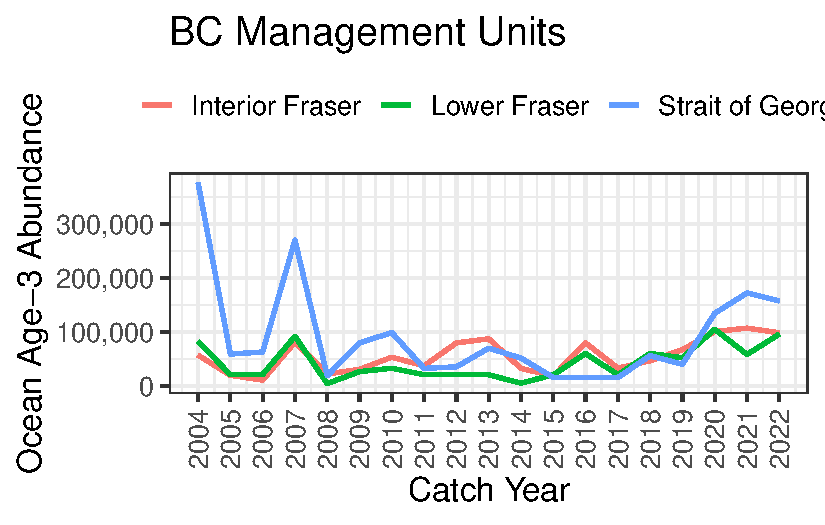
\includegraphics{index-5yr_files/figure-pdf/unnamed-chunk-1-1.pdf}

\textbf{Estimated Post-season Ocean Age-3 Abundances of BC Coho Salmon
Management Units}

\textbf{Estimated Post-season Ocean Age-3 Abundances of US Inside Coho
Salmon Management Units}

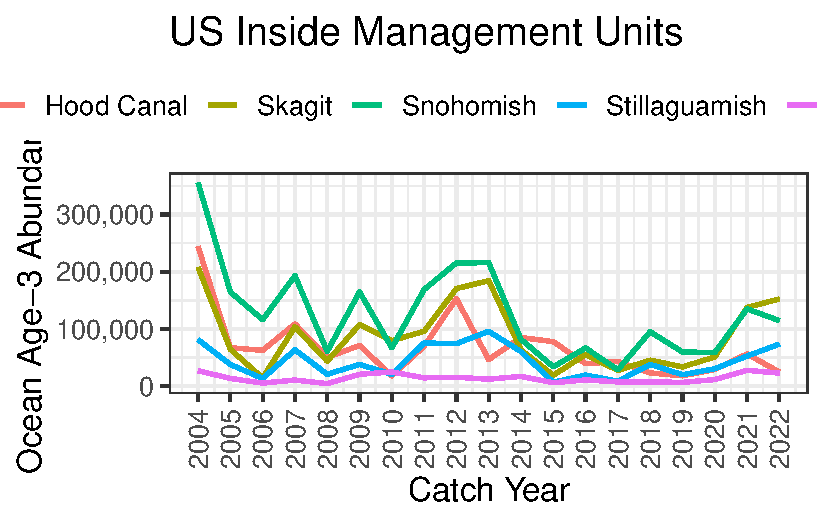
\includegraphics{index-5yr_files/figure-pdf/unnamed-chunk-2-1.pdf}

\textbf{Estimated Post-season Ocean Age-3 Abundances of US Outside Coho
Salmon Management Units}

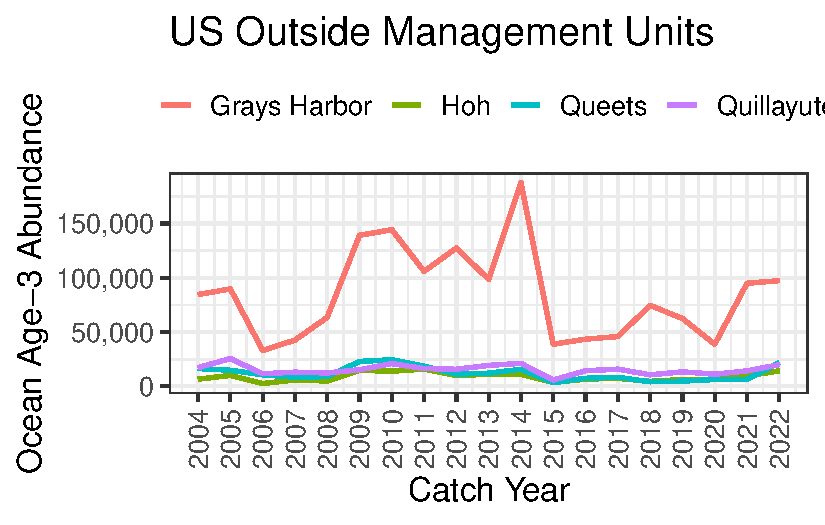
\includegraphics{index-5yr_files/figure-pdf/unnamed-chunk-3-1.pdf}

\textbf{Summary of the number of MUs in each abundance category, based
on post-season assessments.}

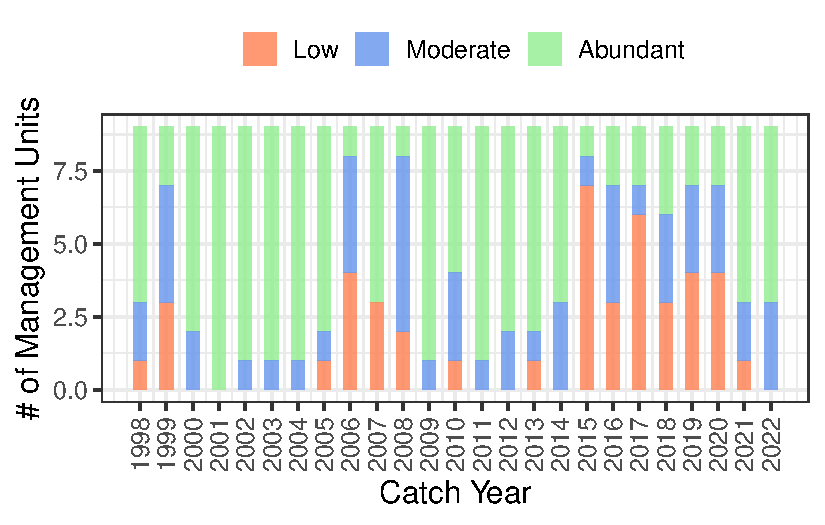
\includegraphics{index-5yr_files/figure-pdf/unnamed-chunk-4-1.pdf}

\subsubsection{Fishery Exploitaion Rate
Overview}\label{fishery-exploitaion-rate-overview}

\textbf{Total exploitation rates by MU.} (note - need to move Canadian
MUs to top of table)

\begin{table}
\fontsize{12.0pt}{14.4pt}\selectfont
\begin{tabular*}{\linewidth}{@{\extracolsep{\fill}}lrrrr}
\toprule
PSC\_StockName & 2019 & 2020 & 2021 & 2022 \\ 
\midrule\addlinespace[2.5pt]
\multicolumn{5}{l}{US Inside} \\[2.5pt] 
\midrule\addlinespace[2.5pt]
Skagit & 48.2\% & 42.6\% & 32.6\% & 25.6\% \\ 
Stillaguamish & 20.3\% & 12.6\% & 10.6\% & 9.9\% \\ 
Snohomish & 17.2\% & 10.6\% & 11.2\% & 8.1\% \\ 
Hood Canal & 46.1\% & 28.7\% & 24.8\% & 54.1\% \\ 
US Strait JDF & 12.0\% & 7.1\% & 7.1\% & 7.7\% \\ 
\midrule\addlinespace[2.5pt]
\multicolumn{5}{l}{US Outside} \\[2.5pt] 
\midrule\addlinespace[2.5pt]
Quillayute & 37.2\% & 17.2\% & 3.7\% & 18.8\% \\ 
Hoh & 56.6\% & 49.2\% & 17.9\% & 30.4\% \\ 
Queets & 41.3\% & 41.8\% & 9.7\% & 30.1\% \\ 
Grays Harbor & 39.6\% & 28.6\% & 22.4\% & 28.8\% \\ 
\midrule\addlinespace[2.5pt]
\multicolumn{5}{l}{Canada} \\[2.5pt] 
\midrule\addlinespace[2.5pt]
Lower Fraser & 14.0\% & 9.6\% & 7.7\% & 10.3\% \\ 
Interior Fraser & 20.0\% & 13.4\% & 9.5\% & 12.4\% \\ 
Strait of Georgia & 16.2\% & 7.4\% & 6.5\% & 8.8\% \\ 
\bottomrule
\end{tabular*}
\end{table}

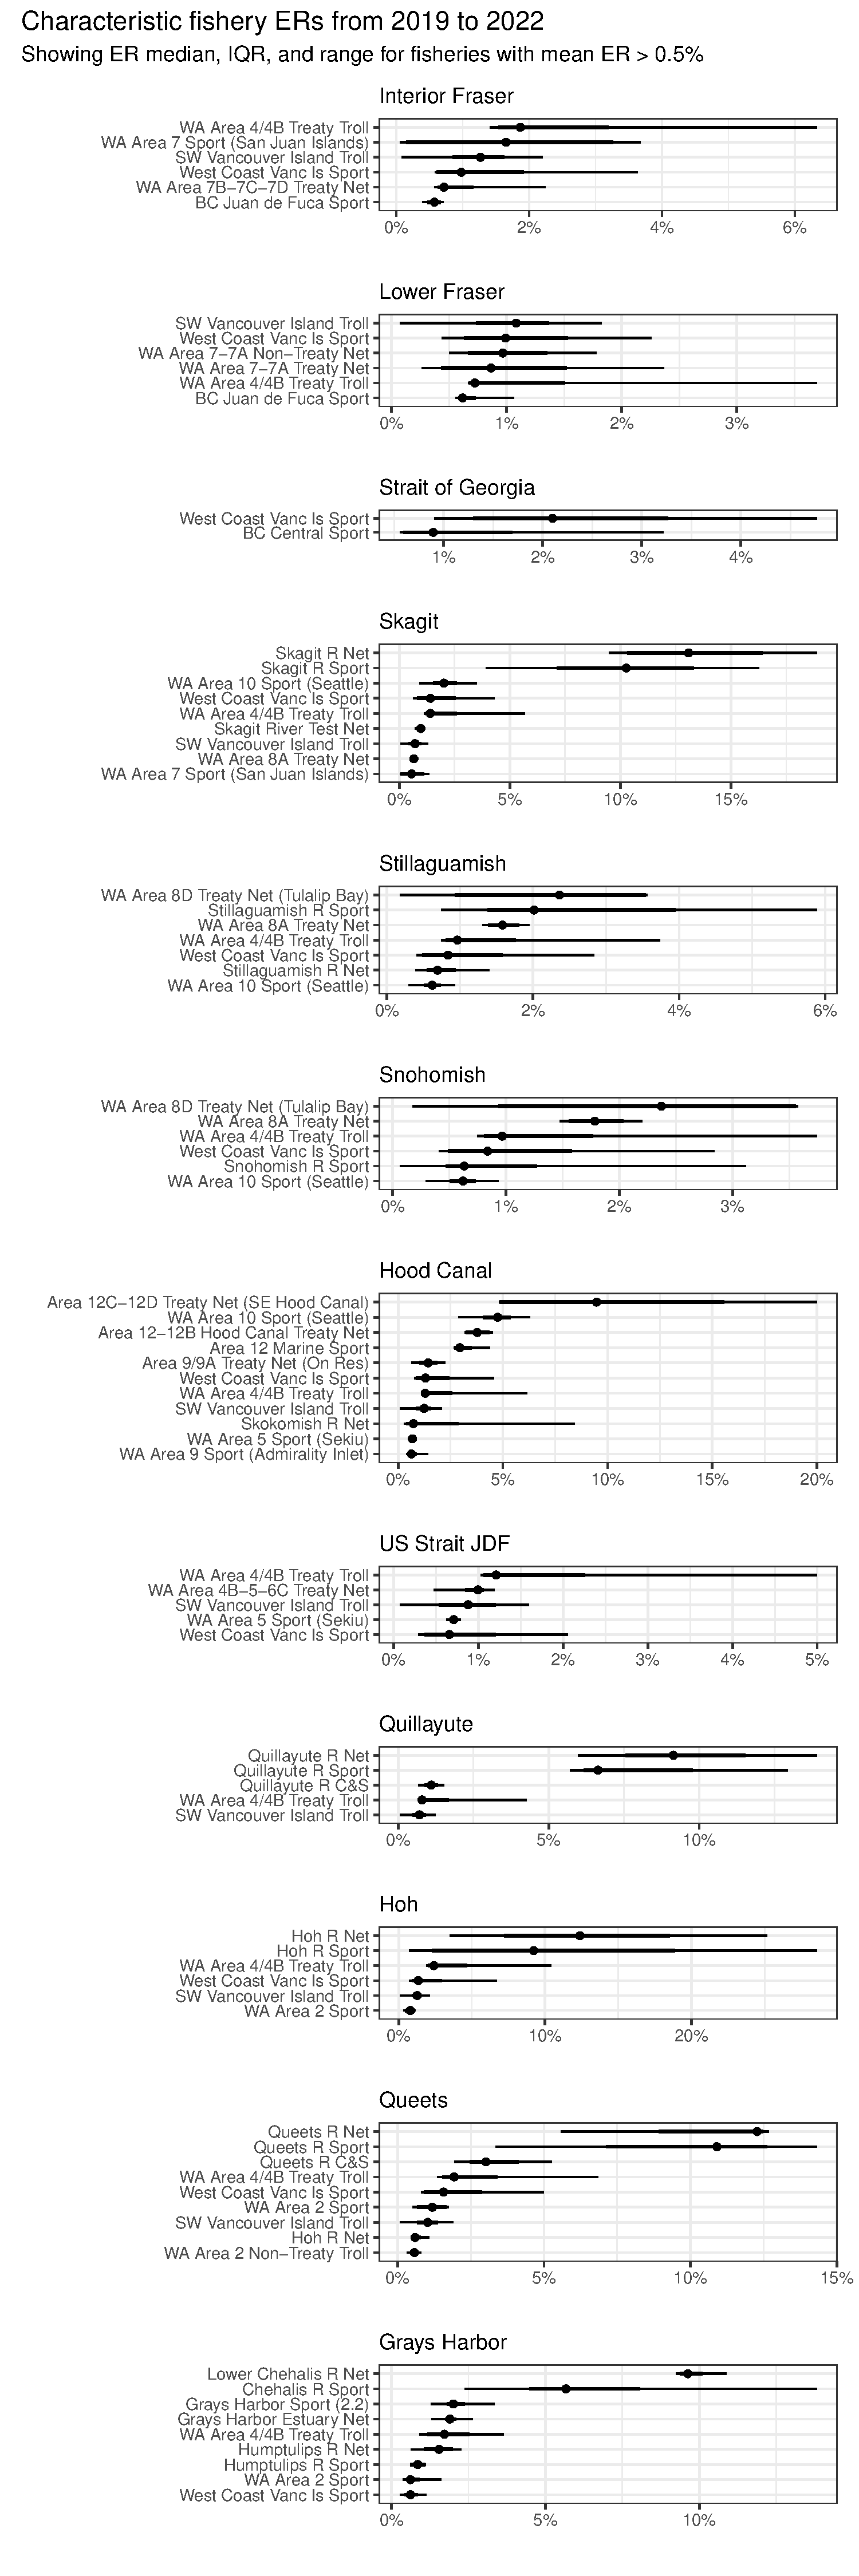
\includegraphics{index-5yr_files/figure-pdf/fishery_er_quantiles-1.pdf}

\subsubsection{Forecast Performance}\label{forecast-performance}

Forecasts are integral to Coho Salmon management in the Pacific
Northwest. These forecasts, as described earlier, are used in pre-season
assessments to determine allowable fishing mortality on stocks of
concern. In the absence of in-season management controls, forecasts that
are too high may yield higher than agreed to exploitation of management
units of concern. Forecasts that are too low may yield losses in fishing
opportunities. The following plots summarize how well preseason
forecasts matched the abundance category (Low, Moderate, Abundance)
identified in post-season runs.

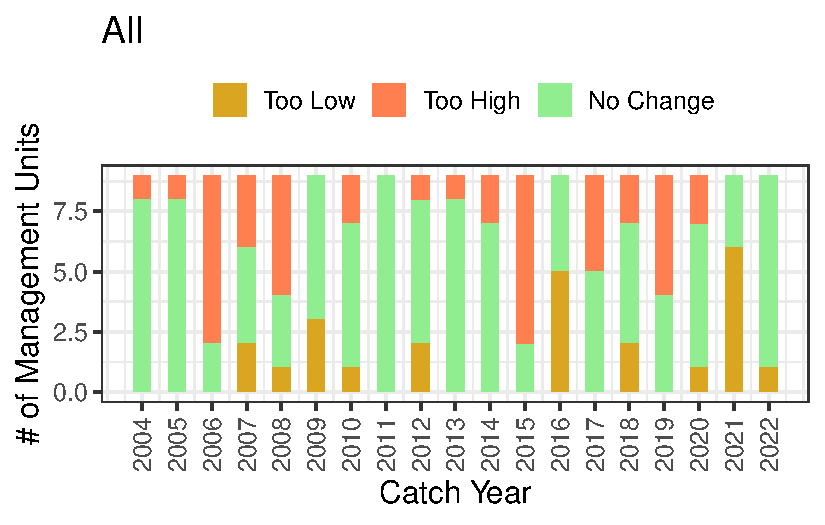
\includegraphics{index-5yr_files/figure-pdf/unnamed-chunk-5-1.pdf}

The following figures provide similar summaries for individual PSC
region.

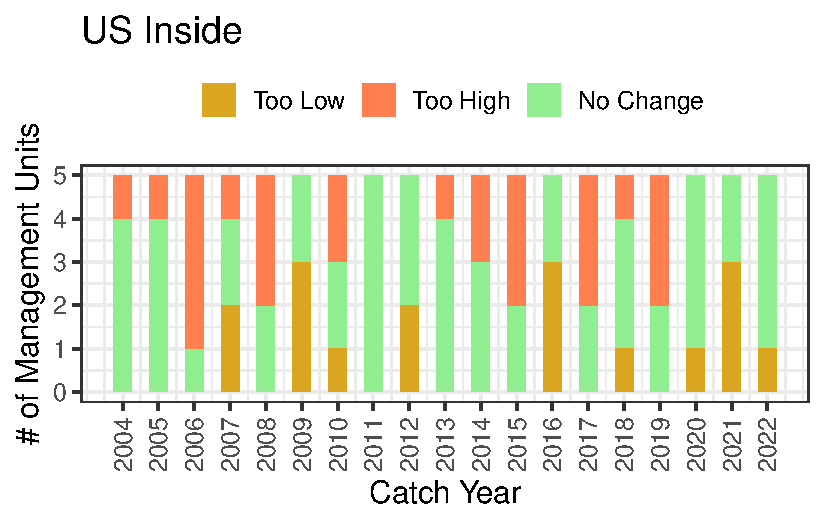
\includegraphics{index-5yr_files/figure-pdf/unnamed-chunk-6-1.pdf}

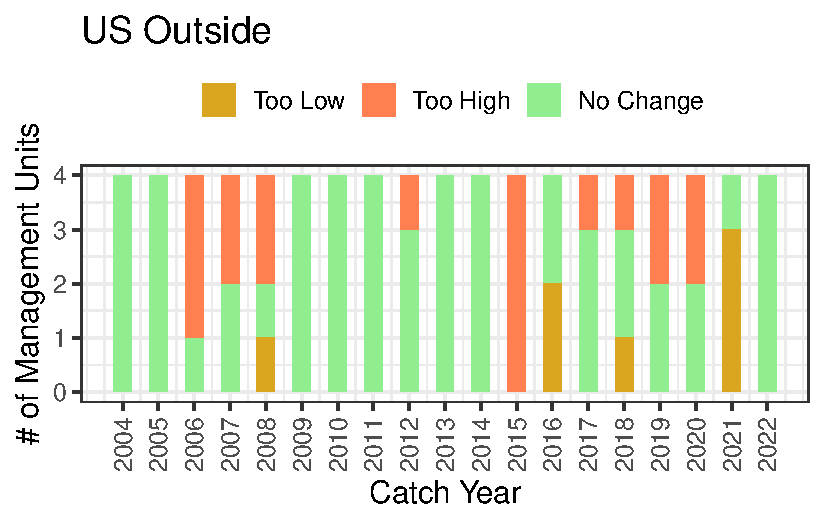
\includegraphics{index-5yr_files/figure-pdf/unnamed-chunk-7-1.pdf}

\section{Was ER under the limits?}\label{was-er-under-the-limits}

Outside limits need to be calculated by hand. For now, just doing inside
management units.

\texttt{Postseason\ Unused\ Using\ Preseason\ Cap} compares how well
Postseason ER would have met the Preseason cap. This removes the effects
of shifts in the abundance category between pre and post-season (if the
abundance category remained the same,
\texttt{Postseason\ Unused\ Using\ Preseason\ Cap} will be the same as
\texttt{Postseason\ Cap}).

\begin{table}
\fontsize{12.0pt}{14.4pt}\selectfont
\begin{tabular*}{\linewidth}{@{\extracolsep{\fill}}rlrrrrrrr}
\toprule
Catch Year & PSC\_StockName & Preseason Cap & Preseason Model ER & Preseason Unused & Postseason Cap & Postseason Model ER & Postseason Unused & Postseason Unused Using Preseason Cap \\ 
\midrule\addlinespace[2.5pt]
2019 & Skagit & 35.0 & 32.4 & 2.6 & 35.0 & 48.2 & -13.2 & -13.2 \\ 
2019 & Stillaguamish & 50.0 & 22.7 & 27.3 & 35.0 & 20.3 & 14.7 & 29.7 \\ 
2019 & Snohomish & 40.0 & 19.6 & 20.4 & 20.0 & 17.2 & 2.8 & 22.8 \\ 
2019 & Hood Canal & 45.0 & 44.5 & 0.5 & 20.0 & 46.1 & -26.1 & -1.1 \\ 
2019 & US Strait JDF & 20.0 & 8.9 & 11.1 & 20.0 & 12.0 & 8.0 & 8.0 \\ 
2020 & Skagit & 35.0 & 30.0 & 5.0 & 35.0 & 42.6 & -7.6 & -7.6 \\ 
2020 & Stillaguamish & 35.0 & 17.9 & 17.1 & 50.0 & 12.6 & 37.4 & 22.4 \\ 
2020 & Snohomish & 20.0 & 12.8 & 7.2 & 20.0 & 10.6 & 9.4 & 9.4 \\ 
2020 & Hood Canal & 45.0 & 42.4 & 2.6 & 45.0 & 28.7 & 16.3 & 16.3 \\ 
2020 & US Strait JDF & 20.0 & 9.0 & 11.0 & 20.0 & 7.1 & 12.9 & 12.9 \\ 
2021 & Skagit & 35.0 & 32.5 & 2.5 & 60.0 & 32.6 & 27.4 & 2.4 \\ 
2021 & Stillaguamish & 50.0 & 28.7 & 21.3 & 50.0 & 10.6 & 39.4 & 39.4 \\ 
2021 & Snohomish & 40.0 & 28.6 & 11.4 & 40.0 & 11.2 & 28.8 & 28.8 \\ 
2021 & Hood Canal & 45.0 & 43.3 & 1.7 & 65.0 & 24.8 & 40.2 & 20.2 \\ 
2021 & US Strait JDF & 20.0 & 9.1 & 10.9 & 40.0 & 7.1 & 32.9 & 12.9 \\ 
2022 & Skagit & 60.0 & 39.5 & 20.5 & 60.0 & 25.6 & 34.4 & 34.4 \\ 
2022 & Stillaguamish & 50.0 & 36.1 & 13.9 & 50.0 & 9.9 & 40.1 & 40.1 \\ 
2022 & Snohomish & 40.0 & 33.7 & 6.3 & 40.0 & 8.1 & 31.9 & 31.9 \\ 
2022 & Hood Canal & 45.0 & 44.3 & 0.7 & 45.0 & 54.1 & -9.1 & -9.1 \\ 
2022 & US Strait JDF & 20.0 & 10.9 & 9.1 & 40.0 & 7.7 & 32.3 & 12.3 \\ 
\bottomrule
\end{tabular*}
\end{table}

\section{Acronyms}\label{acronyms}

\begin{table}
\fontsize{12.0pt}{14.4pt}\selectfont
\begin{tabular*}{\linewidth}{@{\extracolsep{\fill}}lll}
\toprule
Acronym & Definition & URL \\ 
\midrule\addlinespace[2.5pt]
ABM & Abundance-Based Management & <a href="  ">  </a> \\ 
B.C. & British Columbia & <a href="  ">  </a> \\ 
BkFRAM & Backwards FRAM & <a href="  ">  </a> \\ 
BY & Brood Year & <a href="  ">  </a> \\ 
CDFO & Canadian Department of Fisheries and Oceans & <a href=" https://www.dfo-mpo.gc.ca/index-eng.htm "> https://www.dfo-mpo.gc.ca/index-eng.htm </a> \\ 
CFNC & Canadian First Nations Caucus & <a href="  ">  </a> \\ 
CoTC & Coho Joint Technical Committee & <a href=" https://www.psc.org/about-us/structure/committees/technical/coho/ "> https://www.psc.org/about-us/structure/committees/technical/coho/ </a> \\ 
CU & Conservation Unit & <a href=" https://open.canada.ca/data/en/dataset/1ac00a39-4770-443d-8a6b-9656c06df6a3 "> https://open.canada.ca/data/en/dataset/1ac00a39-4770-443d-8a6b-9656c06df6a3 </a> \\ 
CWT & Coded-Wire Tag & <a href=" https://www.nmt.us/cwt/ "> https://www.nmt.us/cwt/ </a> \\ 
DIT & Double-Index Tag & <a href="  ">  </a> \\ 
EDT & Electronic Tag Detection & <a href="  ">  </a> \\ 
ENSO & El Niño-Southern Oscillation & <a href=" https://www.climate.gov/enso "> https://www.climate.gov/enso </a> \\ 
ER & Exploitation Rate & <a href="  ">  </a> \\ 
ESA & U.S. Endangered Species Act & <a href=" https://www.fws.gov/international/laws-treaties-agreements/us-conservation-laws/endangered-species-act.html "> https://www.fws.gov/international/laws-treaties-agreements/us-conservation-laws/endangered-species-act.html </a> \\ 
ESU & Evolutionarily Significant Unit & <a href=" https://www.nwfsc.noaa.gov/assets/4/6878_09172014_172219_Waples.1995.pdf "> https://www.nwfsc.noaa.gov/assets/4/6878_09172014_172219_Waples.1995.pdf </a> \\ 
FMP & Fisheries Management Plan & <a href="  ">  </a> \\ 
FRAFS & Fraser River Aboriginal Fisheries Secretariat & <a href=" https://www.frafs.ca/ "> https://www.frafs.ca/ </a> \\ 
FRAM & Fishery Regulation and Assessment Model & <a href=" https://framverse.github.io/fram_doc/ "> https://framverse.github.io/fram_doc/ </a> \\ 
HC & Hood Canal & <a href="  ">  </a> \\ 
IFMP & Integrated Fisheries Management Plan & <a href=" https://www.pac.dfo-mpo.gc.ca/fm-gp/ifmp-eng.html#Salmon "> https://www.pac.dfo-mpo.gc.ca/fm-gp/ifmp-eng.html#Salmon </a> \\ 
IFR & Interior Fraser River & <a href="  ">  </a> \\ 
iREC & Internet-based Recreational Fishery & <a href=" https://www.pac.dfo-mpo.gc.ca/fm-gp/rec/irec-info-eng.html "> https://www.pac.dfo-mpo.gc.ca/fm-gp/rec/irec-info-eng.html </a> \\ 
JA3 & January Age-3 & <a href="  ">  </a> \\ 
LFFA & Lower Fraser Fishery Alliance & <a href=" https://www.lffa.ca/ "> https://www.lffa.ca/ </a> \\ 
LWFR & Lower Fraser River & <a href="  ">  </a> \\ 
MFMT & Maximum Fishing Mortality Threshold & <a href="  ">  </a> \\ 
MMFN & Mowachaht-Muchalaht First Nation & <a href=" https://www.yuquot.ca/ "> https://www.yuquot.ca/ </a> \\ 
MSF & Mark-Selective Fishery & <a href=" https://wdfw.wa.gov/sites/default/files/about/commission/meetings/2018/08/aug0918_fc_selective_fisheries.pdf "> https://wdfw.wa.gov/sites/default/files/about/commission/meetings/2018/08/aug0918_fc_selective_fisheries.pdf </a> \\ 
MSH & Maximum Sustainable Harvest & <a href=" https://www.pcouncil.org/fact-sheet-annual-catch-limits-and-other-management-thresholds/#:~:text=The%20overfishing%20limit%20(OFL)%20is,the%20FMSY%20harvest%20rate. "> https://www.pcouncil.org/fact-sheet-annual-catch-limits-and-other-management-thresholds/#:~:text=The%20overfishing%20limit%20(OFL)%20is,the%20FMSY%20harvest%20rate. </a> \\ 
MSM & Mixed-Stock Model & <a href="  ">  </a> \\ 
MU & Management Unit & <a href="  ">  </a> \\ 
NMFS & National Marine Fisheries Service & <a href=" https://www.fisheries.noaa.gov/ "> https://www.fisheries.noaa.gov/ </a> \\ 
NOF & North of Falcon & <a href=" https://wdfw.wa.gov/fishing/management/north-falcon "> https://wdfw.wa.gov/fishing/management/north-falcon </a> \\ 
NSF & Non-Selective Fishery & <a href="  ">  </a> \\ 
NTC & Nuu-chah-nulth Tribal Council & <a href=" https://nuuchahnulth.org/ "> https://nuuchahnulth.org/ </a> \\ 
NWIFC & Northwest Indian Fisheries Commission & <a href=" https://nwifc.org/ "> https://nwifc.org/ </a> \\ 
OA3 & Ocean Age-3 & <a href="  ">  </a> \\ 
ODFW & Oregon Department of Fish and Wildlife & <a href=" https://www.dfw.state.or.us/ "> https://www.dfw.state.or.us/ </a> \\ 
OFL & Overfishing Limit & <a href=" https://www.pcouncil.org/fact-sheet-annual-catch-limits-and-other-management-thresholds/#:~:text=The%20overfishing%20limit%20(OFL)%20is,the%20FMSY%20harvest%20rate. "> https://www.pcouncil.org/fact-sheet-annual-catch-limits-and-other-management-thresholds/#:~:text=The%20overfishing%20limit%20(OFL)%20is,the%20FMSY%20harvest%20rate. </a> \\ 
OR & Oregon & <a href="  ">  </a> \\ 
PDO & Pacific Decadal Oscillation & <a href=" https://www.ncei.noaa.gov/access/monitoring/pdo/ "> https://www.ncei.noaa.gov/access/monitoring/pdo/ </a> \\ 
PEF & Production Expansion Factor & <a href="  ">  </a> \\ 
PFMC & Pacific Fisheries Management Council U.S. & <a href=" https://www.pcouncil.org/ "> https://www.pcouncil.org/ </a> \\ 
PS & Puget Sound & <a href=" https://en.wikipedia.org/wiki/Puget_Sound "> https://en.wikipedia.org/wiki/Puget_Sound </a> \\ 
PSC & Pacific Salmon Commission & <a href=" https://www.psc.org/ "> https://www.psc.org/ </a> \\ 
PST & Pacific Salmon Treaty & <a href=" https://www.psc.org/publications/pacific-salmon-treaty/ "> https://www.psc.org/publications/pacific-salmon-treaty/ </a> \\ 
QIN & Quinault Indian Nation & <a href=" http://www.quinaultindiannation.com/ "> http://www.quinaultindiannation.com/ </a> \\ 
RMIS & Regional Mark Information System & <a href=" https://www.rmpc.org/ "> https://www.rmpc.org/ </a> \\ 
RMISD & Regional Mark Information System Database (U.S.) & <a href=" https://www.rmpc.org/ "> https://www.rmpc.org/ </a> \\ 
RMPC & Regional Mark Processing Center & <a href=" https://www.rmpc.org/ "> https://www.rmpc.org/ </a> \\ 
RRTERM & Terminal Area Run Reconstruction Program & <a href="  ">  </a> \\ 
SCMP & Southern Coho Management Plan & <a href=" https://www.psc.org/publications/pacific-salmon-treaty/ "> https://www.psc.org/publications/pacific-salmon-treaty/ </a> \\ 
SRSC & Skagit River System Cooperative & <a href="  ">  </a> \\ 
SIT & Single Index Tag & <a href="  ">  </a> \\ 
SJDF & Strait of Juan de Fuca & <a href="  ">  </a> \\ 
SUQ & Suquamish Tribe & <a href=" https://suquamish.nsn.us/ "> https://suquamish.nsn.us/ </a> \\ 
TT & Tulalip Tribes & <a href=" https://www.tulaliptribes-nsn.gov/ "> https://www.tulaliptribes-nsn.gov/ </a> \\ 
U.S. & United States & <a href="  ">  </a> \\ 
UFFCA & Upper Fraser Fisheries Conservation Alliance & <a href=" https://www.upperfraser.ca/ "> https://www.upperfraser.ca/ </a> \\ 
USFWS & U.S. Fish and Wildlife Service & <a href=" https://www.fws.gov/ "> https://www.fws.gov/ </a> \\ 
WA & Washington & <a href="  ">  </a> \\ 
WCVI & West Coast of Vancouver Island & <a href="  ">  </a> \\ 
WDFW & Washington Department of Fish and Wildlife & <a href=" https://wdfw.wa.gov/ "> https://wdfw.wa.gov/ </a> \\ 
WSP & Wild Salmon Policy (Canada) & <a href="  ">  </a> \\ 
WRIA & Water Resource Inventory Area (U.S.) & <a href="  ">  </a> \\ 
\bottomrule
\end{tabular*}
\end{table}

\section{Glossary}\label{glossary}

\begin{table}
\fontsize{12.0pt}{14.4pt}\selectfont
\begin{tabular*}{\linewidth}{@{\extracolsep{\fill}}ll}
\toprule
Term & Definition \\ 
\midrule\addlinespace[2.5pt]
Abundance-Based Management (ABM) & A management framework that constrains exploitation rates, based on a categorical abundance forecast (abundant, moderate, low) for naturally-spawning Coho Management Units. The purpose is to provide more protection when the status of the fish is low and the conservation need is greatest, and more harvest opportunity when abundance is high. Exploitation rate caps are specified in the Pacific Salmon Treaty Southern Coho Agreement. \\ 
Base Period (FRAM) & The FRAM base period is a period chosen to represent average temporal and geographic distributions of Coho Salmon coastwide. The base period was developed by summarizing coded-wire-tag information from a continuous time period containing a sufficient number of CWT releases and fishery recoveries. The current Coho base period is comprised of CWT recoveries from catch years 1986–1992. The Mixed-stock Model (MSM) and cohort reconstruction methods were used to estimate base period exploitation rates and other parameters, such as base period cohort sizes and fishery compositions, for all FRAM stocks and fisheries by time step. The base period is made up of the averages of these estimates over the catch years 1986 through 1992. Using these base period parameters allows FRAM to predict the stock composition, exploitation rates, and escapements of future fisheries when provided with forecasts of abundance and fishery mortalities. \\ 
Break point & A Management Unit-specific ocean age-3 abundance level that determines the categorical status of a stock (i.e., abundant, moderate, low). \\ 
Brood Year (BY) & The year in which the majority of parent fish spawned and deposited fertilized eggs. \\ 
By-catch & Incidental or unintentional catch of non-target stocks or species. \\ 
Catch & The number of fish that are retained in a fishery. \\ 
Coded-Wire Tag (CWT) & A small piece of magnetized stainless-steel wire that is injected into the snout of a juvenile salmon (usually hatchery stock). Each tag is 0.25 mm in diameter and typically 1.1 mm long and is etched with a code that identifies its specific release group. Each code is associated with release information, including date and location of release, hatchery, stock, fish size, and number of fish tagged with that same code (referred to as a release group). Tags are typically recovered from returning adults through fishery and escapement sampling. Release and recovery Information is stored in the U.S. in the Regional Mark Information System's (RMIS) Release database and in Canada’s Mark Recovery Program. \\ 
Cohort & A group of fish belonging to the same brood year. \\ 
Cohort Abundance & For each stock unit, an annual abundance is obtained from a regional expert, typically in the form of an ocean age-3 run size (pre-fishing age-3 abundance in the ocean after natural mortality has been subtracted). In a pre-season context these abundances come from annual forecasts, whereas in a post-season context the abundances are derived from estimates of actual returns. For Coho, an initial stock abundance is needed for adult fish (age-3) by mark status. \\ 
Cohort Reconstruction or Cohort Analysis & Cohort reconstruction is a method commonly used in salmon stock assessment for estimation of exploitation rates. The basic principle of cohort reconstruction is the sequential estimation of a cohort’s abundance from the end of the cohort’s life span, when abundance is zero, to a specified earlier age (commonly age-3 for Coho). A full cohort reconstruction can be completed only once the cohort’s life span has ended. Age-specific escapement and harvest data are required and, in general, the natural mortality rates are assumed. \\ 
Co-management & The collaborative process between co-managers–tribal governments and state governments on the West Coast. Using scientific information, the co-managers make decisions about the management of fisheries to ensure that the fisheries meet legal requirements, treaty fishing rights, and conservation goals. \\ 
Command Files & The files used in the Fisheries Regulation Assessment Model containing all the necessary input parameters to run the model, such as forecasted abundance estimates and fishery regulations. A separate command file is developed for each FRAM run. \\ 
Conservation Unit (CU) & Salmon populations that have been identified as distinct units of biodiversity under the Canadian Wild Salmon Policy (see Holtby and Ciruna 2007). A Conservation Unit (CU) is a group of wild Pacific salmon sufficiently isolated from other groups that, if extirpated, is very unlikely to recolonize naturally within an acceptable timeframe, such as a human lifetime or a specified number of salmon generations. \\ 
Double-Index Tag (DIT) & Paired groups of tagged fish, each tagged with separate CWT tag code, used to determine differential exploitation rates on marked and unmarked fish subjected to mark-selective fisheries. Both groups are presumed identical except that one group is externally marked (adipose fin clipped) and one group is unmarked (not adipose fin clipped). \\ 
El Niño Index (ONI) & The Oceanic Niño Index (ONI) is an index for tracking the ocean part of ENSO, the El Niño-Southern Oscillation climate pattern. The ONI is a rolling 3-month average temperature anomaly in the surface waters of the east-central tropical Pacific, near the International Dateline. Index values of +0.5 or higher indicate El Niño. Values of -0.5 or lower indicate La Niña. \\ 
Electronic Tag Detection (ETD) & The use of a handheld wand or tunnel type detector that can sense the magnetized coded-wire tag within a fish's snout. \\ 
Endangered Species Act  (U.S.) & The Endangered Species Act (ESA) is the primary law in the United States for protecting critically important species that are at risk of extinction. Under the ESA, the federal government has the responsibility to protect these species and their critical habitats. NOAA Fisheries is responsible for endangered and threatened salmon. \\ 
Enhancement & Use of hatcheries, spawning channels, lake fertilization or habitat restoration to increase the survival rate or production of salmon at some stage of its life. \\ 
Escapement (Spawning Escapement) & The number of adult salmon that escape all fisheries and other forms of mortality to return to a hatchery or stream to spawn. \\ 
Evolutionarily Significant Unit (ESU) & Under the U.S. Endangered Species Act, a group of Pacific salmon populations that represent an important component of the evolutionary legacy of the species and are therefore treated as a single “species”. \\ 
Exclusive Economic Zone & The Exclusive Economic Zone (EEZ) is an area from 3 to 200 nautical miles offshore of coastal states and is classified as federal waters. In the EEZ, the U.S. has special rights about the exploration and use of marine resources, which includes energy production from water and wind, and fisheries. \\ 
Exploitation Rate (ER) & Expressed as a percentage, the proportion of the total return of adult salmon in a given year that die as a result of fishing activity. Mortalities include landed catch and incidental mortalities. \\ 
Exploitation Rate Cap & The maximum exploitation rate an MU can be subjected to given its categorical abundance status. Under the ABM, allowable exploitation rate is shared by Canada and the U.S. \\ 
Fisheries Management & Fisheries management is a process that relies on science, management approaches, enforcement, partnerships, and public participation. Fisheries management uses scientific information (e.g., number of fish caught, types of fish caught, life cycle knowledge) and input from fishing communities to help guide management decisions and conservation objectives. \\ 
Fisheries Management Plan (FMP) & The set of fisheries planned to distribute exploitation rates amongst fisheries and time periods each year. These are termed Integrated Fisheries Management Plans in Canada. \\ 
Fishery & A fishery is an activity leading to the harvesting of fish and can be specified by the species of fish caught, people involved, location, method of fishing, and purpose of the activities. Fish caught in a fishery can be for commercial, recreational, or tribal and ceremonial purposes. \\ 
Fishery Regulation Assessment Model (FRAM) & A model used to estimate the MU- and fishery-specific impacts. The Forwards FRAM projects MU-specific mortalities and escapements under proposed fishery regimes given pre-season forecasts. The Backwards Coho FRAM estimates unspecified MU abundances using estimates of escapements and fishing mortalities. It includes 246 stocks, 198 fisheries, and 5 time steps. \\ 
Fry & Salmon that have emerged from gravel, completed yolk absorption, remained in freshwater streams, and are less than a few months old. \\ 
FSC (Canada) & First Nations' fishery for food, social, and ceremonial use. \\ 
Harvest & The term harvest refers to the total number of fish caught and kept from an area or fishery during a period of time. \\ 
Incidental mortality & Mortality incurred during fishing  in addition to landed catch. For example, some fish die as a result of being caught and released. \\ 
Indicator stock & A coded-wire-tagged surrogate stock that is used to make inferences for a particular MU. For example, a CWT release from a hatchery stock may be used to estimate the distribution and magnitude of fishing mortalities. \\ 
Integrated Fisheries Management Plan (IFMP) & These Canadian plans identify the main objectives and requirements for Pacific fisheries and outline the management to achieve these objectives. IFMPs provide a common understanding of the basic rules for the sustainable management of the fisheries resource, and communicate basic information about fish stocks and our fisheries. \\ 
Interception & Interception occurs when a salmon from one state or country is caught in another state or country's fisheries. As salmon grow and mature in the Pacific Ocean, they travel along the West Coast and across international borders. Salmon that originate in U.S. streams may migrate through Canadian waters, where they may be caught in Canadian fisheries. Salmon from Oregon streams can be caught in Washington fisheries. \\ 
January age-3 abundance (JA3) & The estimated abundance of fish of age-3 (adults) in January before any fisheries start. January age-3 abundance is estimated as fishing mortality plus escapement plus natural mortality. \\ 
La Niña &  \\ 
Landed catch & Fish that are caught and kept (see Incidental mortality) \\ 
Magnuson-Stevens Fishery Conservation and Management Act (MSA) & The Magnuson-Stevens Fishery Conservation and Management Act (MSA) is the primary law that governs fisheries management in the federal marine waters (3-200 miles offshore) of the United States. The goal of the MSA is to encourage the long-term biological and economic sustainability of marine fisheries. \\ 
Management Unit (MU) & Under the PST Southern Coho agreement, a geographically-based aggregate of salmon populations, that is managed under a single set of exploitation rate caps. \\ 
Mark-Selective Fishery (MSF) & A fishery that requires marked fish (i.e., those with adipose fin clips) and unmarked fish (those with intact adipose fins) to be differentially retained (e.g., marked fish kept, unmarked fish released). \\ 
Maximum Sustainable Harvest (MSH) & An estimate of the largest average annual catch or yield that can be continuously taken over a long period from a stock under prevailing ecological and environmental conditions. \\ 
Mixed-Stock Model & A model used to estimate the cohort abundances in mixed stock fisheries using coded-wire tags and estimates of catch (see Production Expansion Factors). \\ 
Naturally Produced & Originated from spawning in the natural environment, as opposed to spawned in a hatchery. Often considered “wild”. \\ 
Non-retention fisheries & Fisheries in which a particular group of fish are not allowed to be kept (e.g., due to species or external marks) (see Retention Fisheries) \\ 
Non-selective fisheries (NSF) & Fisheries allowed to retain both marked (adipose fin clipped) and unmarked fish (see Mark-selective fishery). \\ 
North of Falcon & Each year state, federal, and tribal fishery managers gather to plan the Northwest's recreational and commercial salmon fisheries. This series of meetings – involving representatives from federal, state and tribal governments and recreational and commercial fishing industries – is known as the North of Falcon process. The North of Falcon planning process coincides with the March and April meetings of the Pacific Fishery Management Council (PMFC), the federal authority responsible for setting ocean salmon seasons 3 to 200 miles off the Pacific coast. In addition to the two PFMC meetings, the states of Washington and Oregon and the Treaty Tribes sponsor additional meetings to discuss alternative fishing seasons that meet conservation and allocation objectives. Fishery managers generally refer to the entire set of pre-season meetings as North of Falcon. The name refers to Cape Falcon in northern Oregon, which marks the southern border of active management for Washington salmon stocks. \\ 
Ocean Age-3 Abundance (OA3) & Total number of fish that are harvested (including incidental mortality) plus those that escape to spawn (also referred to as “cohort abundance” or “ocean recruits”). Natural mortality is not included. This abundance status of a Management Unit is based upon this estimate of abundance. \\ 
Overfishing Limit (OFL) & The overfishing limit (OFL) is the maximum amount of a stock that can be caught in a year without resulting in overfishing. Groundfish OFLs for assessed stocks are typically determined by multiplying the estimated abundance of the exploitable biomass of a stock by the FMSY harvest rate. There are also methods for determining OFLs for unassessed stocks. Setting OFLs is a scientific (as opposed to policy) determination made by the Scientific and Statistical Committee (SSC). OFLs are set for every actively managed stock or stock complex. \\ 
Pacific Decadal Oscillation (PDO) & The PDO describes the pattern of sea surface temperatures around the North Pacific Ocean north of 20°N.  During a "warm", or "positive", phase, the west Pacific becomes cooler and part of the eastern ocean warms; during a "cool", or "negative", phase, the opposite pattern occurs.  The index was originally described by Mantua et al. 1997 (Bulletin of the American Meteorological Society. 78 (6): 1069–79.) \\ 
Pacific Salmon Commission (PSC) & A joint Canada/U.S. commission established under the Pacific Salmon Treaty to oversee the implementation of the Pacific Salmon Treaty. \\ 
Pacific Salmon Treaty (PST) & A treaty between Canada and the United States concerning the conservation, management, restoration, and enhancement of pacific salmon resources. \\ 
Pacific States Marine Fisheries Commission  (PSMFC) & Pacific States Marine Fisheries Commission (PSMFC) is a non‐regulatory agency that serves Alaska, California, Idaho, Oregon, and Washington. PSMFC (headquartered in Portland) administers salmon disaster relief funds, provides a communication exchange between the Pacific Fishery Management Council and the North Pacific Fishery Management Council, and provides information in the form of data services for various fisheries. \\ 
Production Expansion Factor (PEF) & A scalar that represents the number of fish in a population from a single CWT recovery. \\ 
Rebuilding & The process of rebuilding an overfished stock. For salmon, rebuilding usually takes the form of reduced harvest limits. \\ 
Reference Point & A Management Unit-specific ocean age-3 abundance level that determines the categorical status of a stock (i.e., abundant, moderate, low). \\ 
Regional Mark Information System (RMIS) & Database containing data on salmonid releases, recoveries in fisheries and escapement, and estimated catch by fishery and time period. \\ 
Retention fisheries & Fisheries in which fish of a particular group are allowed to be kept (see Non-retention fisheries). \\ 
Return year & The year in which fish would normally return to spawn as adults. For Southern Coho Salmon that mature as 3 year old adults, return year is Brood Year + 3. \\ 
RR Term & A program that reconstructs terminal Coho runs using freshwater and terminal area marine fisheries and escapement data for Puget Sound stocks. \\ 
Run & As salmon migrate back to freshwater as adults, they arrive in groups called runs, which are typically associated with a season (spring, summer, fall, winter). A run of salmon may be composed of salmon from a single age or multiple ages, and can be from a single stock or multiple stocks. \\ 
Sibling Forecast & In all species of Pacific salmon but pinks, the individual salmon produced in any one spawning year mature and return to spawn in more than one subsequent year. All of the fish that return from a spawning year (the brood year) are collectively referred to as a cohort or the brood-year return. A sibling forecast uses the first returns from a cohort to predict the number of their siblings that will return in subsequent years. Generally, the first year of return is dominated by males and the last year of returns by females. \\ 
Single Index Tag (SIT) & A group of coded-wire-tagged (CWT) fish that are not paired with another release group. They can be marked (clipped) or unmarked (unclipped). \\ 
Smolt & A smolt is a life cycle phase of a salmon or steelhead when the fish is preparing for the transition from freshwater to saltwater. The process is called smoltification. A smolt becomes physiologically capable of balancing salt and water in the estuary and ocean waters. Smolts vary in size and age depending on the species of salmon. \\ 
Smolt Year & The year in which fish would normally enter the ocean as smolts.  For Southern Coho Salmon, smolt year is brood year + 2 and return year − 1.  Often described as “smolt outmigration year”. \\ 
Southern Coho Management Plan (SCMP) & An agreement between the U.S. and Canada that specifies how the Parties’ fisheries impact on Coho Salmon that originate in southern British Columbia, Washington and Oregon shall be managed, subject to future approved technical refinements. It is described in Annex IV, Chapter 5 of the current Pacific Salmon Treaty. \\ 
Spawning Escapement & The number of adult fish that “escape” fisheries and return to freshwater to spawn. \\ 
Spawning Grounds/Spawn & Spawning grounds are the freshwater areas where salmon and steelhead spawn. \\ 
Special management zone (SMZ) & Geographic/temporal areas in B.C. that have special management restrictions. \\ 
Status & A Management Unit's status (Low, Moderate, and Abundant) is based on its forecasted (pre-season) or estimated (post-season) ocean Age-3 abundance. \\ 
Stock & A group of interbreeding organisms that is relatively isolated (i.e., demographically uncoupled) from other such groups and is likely adapted to the local habitat. Fish species are made up of an aggregate of stocks. \\ 
Stock Assessment & The use of various statistical and mathematical calculations to make quantitative predictions about the reactions of fish populations to alternative management choices. \\ 
Subsistence Fisheries & In the Pacific Northwest of the U.S., the term "Ceremonial and Subsistence" (C\&S) is used to describe non-commercial harvest in Treaty Tribe fisheries for personal, ritual, or community use. In Canada, the term "Food, Social, and Ceremonial" (FSC) is used to describe the non-commercial harvest of fish by the First Nations. \\ 
Treaty/Treaties & A treaty is a formal, legally binding agreement that establishes obligations between and among two or more countries, states, or sovereign nations. Examples of treaties include the Pacific Salmon Treaty and treaties between the U.S. and American Indian Tribes. \\ 
Troll Fishery (Trolling) & Fishing with a hook or hooks attached to a line that is towed through the water or from a vessel. Commercial trollers employ hooks and lines that are suspended from large poles extending from the fishing vessel \\ 
Voluntary Head Recovery Program (VHRP) & A sampling program in B.C. for recreational fisheries that relies upon anglers voluntarily returning heads from marked salmon so CWTs may be recovered. \\ 
Wild Salmon & Salmon are considered "wild" if they have spent their entire life cycle in the wild and originate from parents that were also produced by natural spawning and continuously lived in the wild. \\ 
\bottomrule
\end{tabular*}
\end{table}

\section{References}\label{references}

\phantomsection\label{refs}
\begin{CSLReferences}{1}{0}
\bibitem[\citeproctext]{ref-PSC_1999}
Pacific Salmon Commission. 1999. {Pacific Salmon Treaty}. Pacific Salmon
Commission, Vancouver, BC.

\bibitem[\citeproctext]{ref-PSC_2009}
Pacific Salmon Commission. 2009. {Pacific Salmon Treaty}. Pacific Salmon
Commission, Vancouver, BC.

\bibitem[\citeproctext]{ref-PSC_2022}
Pacific Salmon Commission. 2022.
\href{https://www.psc.org/publications/pacific-salmon-treaty/}{{Pacific
Salmon Treaty}}. Pacific Salmon Commission, Vancouver, BC.

\bibitem[\citeproctext]{ref-Weitkamp_et_al_1995}
Weitkamp, L. A., T. C. Wainwright, G. J. Bryant, G. B. Milner, D. J.
Teel, R. G. Kope, and R. S. Waples. 1995. {Status review of coho salmon
from Washington, Oregon, and California}. U.S. Department of Commerce,
National Marine Fisheries Service, NOAA Technical Memo NMFS NWFFSC 24.

\end{CSLReferences}

\section{Ref\_older}\label{sec-refs}

\emph{internal inline links direct here, individual refs themselves will
have external links as `(pdf){[}urls\_of\_raw.pdf{]}' for reader to
click}

\section{Appendix: Annual CoTC reports of Estimates of Exploitation
Rates}\label{appendix-annual-cotc-reports-of-estimates-of-exploitation-rates}

\href{https://www.psc.org/publications/technical-reports/technical-committee-reports/coho/}{General
archive of public CoTC reports}

The following provides annual report info without making the individual
files themselves publicly available where they would lack the context of
the Periodic Report.




\end{document}
